\section{Hybrid hyper-reduction for contact}\label{sec:vf-hyb}

\subsection*{Concept and purpose}

\citet{fauque2018hybrid} reduce a frictionless contact problem by keeping the \emph{displacements} in a reduced basis while the contact forces (the Lagrange multipliers) on a reduced integration domain (RID) stay finite element unknowns, which is why the model is called hybrid. Signorini conditions then hold exactly at the contact points of the RID, and no compressed basis of non-negative multipliers is needed. The RID is built from discrete empirical interpolation points of the displacement basis, and a greedy loop driven by a solve-free error indicator chooses the training parameters. The paper tests the method on a one-dimensional rope against an obstacle and on a three-dimensional pellet--cladding problem. The study rebuilds both and compares with the projection-based method of \Cref{sec:vf-bal} (the ``PB'' method) at equal accuracy.

The study uses the contact solvers of \fea{} (\anchor{fea_engine.contact_solvers}) for the full-order problem and the existing \rom{} building blocks (POD, \anchor{rom_engine.deim_indices}, inf-sup enrichment, \anchor{rom_engine.reconstruct_contact_forces}, the PB method with a non-negative dual basis). The hybrid solve itself, with the RID construction, the restricted full-order problem on the RID and the indicator $\eta$, is new code written for this study and now in \rom{} as \anchor{rom_engine.contact_rid} (with eight unit tests).

\subsection*{Mathematics as implemented}

\emph{Full-order problem.} A discretised frictionless contact problem is the saddle-point system
\begin{equation}\label{eq:hb-fom}
\mathbf K\mathbf U+\mathbf B^{T}\boldsymbol\Lambda=\mathbf F,\qquad\mathbf B\mathbf U\le\mathbf D,\qquad\boldsymbol\Lambda\ge\mathbf 0,\qquad\boldsymbol\Lambda\odot(\mathbf B\mathbf U-\mathbf D)=\mathbf 0,
\end{equation}
with $\mathbf K\in\mathbb R^{N\times N}$ the stiffness, $\mathbf B$ the gap matrix, $\mathbf D$ the initial gap and $\odot$ the element-wise product. \fea{} uses the opposite sign convention ($\mathbf K\mathbf u=\mathbf f+\mathbf B^{T}\boldsymbol\lambda$, $\mathbf B\mathbf u\ge\mathbf c$), so the scripts call it with $\mathbf B\to-\mathbf I$, $\mathbf c\to-\mathbf D$.

\emph{Basis and RID.} The primal basis $\mathbf V\in\mathbb R^{N\times l_u}$ is a POD of the snapshots, keeping the smallest $l_u$ whose information rate reaches $1-\epsilon_{\rm tol}$,
\begin{equation}\label{eq:hb-rate}
\tau(l_u)=\frac{\sum_{j\le l_u}\sigma_j^2}{\sum_j\sigma_j^2}\ge1-\epsilon_{\rm tol}.
\end{equation}
Discrete empirical interpolation selects $l_u$ indices from $\mathbf V$ (and from a coarse POD of the multiplier snapshots, so that the contact zone is represented); the RID is the union of the element supports of these degrees of freedom, optionally enlarged by rings of neighbouring elements. Let $\mathcal P$ be the degrees of freedom all of whose incident elements lie in the RID (their balance equations can be written exactly there), $\mathcal E$ all degrees of freedom of RID elements, $\Gamma_I=\mathcal E\setminus\mathcal P$ the interface, and $\mathcal C_\lambda$ the contacts whose gap is computable from $\mathcal P$.

\emph{Hybrid reduced problem.} With the enriched basis $\bar{\mathbf V}$ below, the reduced problem is a Petrov--Galerkin system
\begin{equation}\label{eq:hb-red}
\begin{cases}
\bar{\mathbf V}[\mathcal P,:]^{T}\mathbf K[\mathcal P,\mathcal E]\,\bar{\mathbf V}[\mathcal E,:]\,\boldsymbol\gamma+(\mathbf B[\mathcal C_\lambda,:]\bar{\mathbf V})^{T}\boldsymbol\Lambda[\mathcal C_\lambda]=\bar{\mathbf V}[\mathcal P,:]^{T}\mathbf F[\mathcal P],\\[2pt]
\boldsymbol\Lambda[\mathcal C_\lambda]\odot(\mathbf B[\mathcal C_\lambda,:]\bar{\mathbf V}\boldsymbol\gamma-\mathbf D[\mathcal C_\lambda])=\mathbf 0,\quad
\mathbf B[\mathcal C_\lambda,:]\bar{\mathbf V}\boldsymbol\gamma\le\mathbf D[\mathcal C_\lambda],\quad\boldsymbol\Lambda[\mathcal C_\lambda]\ge\mathbf 0 ,
\end{cases}
\end{equation}
with the displacement $\mathbf U=\bar{\mathbf V}\boldsymbol\gamma$ on the whole domain. The reduced matrix $\mathbf A=\bar{\mathbf V}[\mathcal P,:]^{T}\mathbf K[\mathcal P,\mathcal E]\bar{\mathbf V}[\mathcal E,:]$ is not symmetric. Eliminating $\boldsymbol\gamma$ gives the condensed complementarity problem solved online with Lemke's algorithm,
\begin{equation}\label{eq:hb-lcp}
\boldsymbol\gamma=\mathbf A^{-1}(\mathbf b-\mathbf B_r^{T}\boldsymbol\Lambda),\qquad
\mathbf w=(\mathbf D-\mathbf B_r\mathbf A^{-1}\mathbf b)+(\mathbf B_r\mathbf A^{-1}\mathbf B_r^{T})\boldsymbol\Lambda\ge\mathbf 0,\quad\boldsymbol\Lambda\ge\mathbf 0,\quad\boldsymbol\Lambda^{T}\mathbf w=0,
\end{equation}
with $\mathbf b=\bar{\mathbf V}[\mathcal P,:]^{T}\mathbf F[\mathcal P]$ and $\mathbf B_r=\mathbf B[\mathcal C_\lambda,:]\bar{\mathbf V}$; a plain active-set loop on the saddle system \cref{eq:hb-red} picks wrong contact sets ($\operatorname{cond}(\mathbf A)\approx10^{14}$).

\emph{Inf-sup condition.} Well-posedness needs $\mathbf B_r$ to have full row rank (a necessary condition is $\bar l_u\ge N^C_\lambda$). If it fails, unit vectors at contact degrees of freedom are appended,
\begin{equation}\label{eq:hb-enrich}
\bar{\mathbf V}=\big[\mathbf V\ \big|\ \mathbf I_N[:,i^c_1],\dots,\mathbf I_N[:,i^c_{\bar l_u-l_u}]\big],
\end{equation}
so part of the primal field is treated with full-order functions at the contact degrees of freedom.

\emph{Reconstruction outside the RID.} The reduced model returns $\boldsymbol\Lambda$ only on $\mathcal C_\lambda$; outside it a non-negative least-squares fit over multiplier snapshots $\mathbf S_\lambda$ is used,
\begin{equation}\label{eq:hb-nnls}
\min_{\boldsymbol\gamma_\lambda\ge0}\Big\lVert\begin{pmatrix}\mathbf S_\lambda[\mathcal C_\lambda,:]\\ [\mathbf B\mathbf U-\mathbf D]_{-}\odot\mathbf S_\lambda\end{pmatrix}\boldsymbol\gamma_\lambda-\begin{pmatrix}\boldsymbol\Lambda[\mathcal C_\lambda]\\\mathbf 0\end{pmatrix}\Big\rVert_2^2,\qquad\boldsymbol\Lambda=\mathbf S_\lambda\boldsymbol\gamma_\lambda,
\end{equation}
the first block matching the RID multipliers and the second penalising force where the gap is open.

\emph{Indicator and greedy sampling.} For a new parameter $\mu$ the snapshot displacements on $\Gamma_I$ are interpolated in parameter space, $\tilde{\mathbf U}(\mu)[\Gamma_I]=\sum_\rho\alpha_\rho(\mu)\mathbf U(\rho)[\Gamma_I]$, and the full-order problem written only on the RID is solved with this Dirichlet data,
\begin{equation}\label{eq:hb-restr}
\mathbf K[\mathcal P,\mathcal P]\tilde{\mathbf U}_{\mathcal P}+\mathbf B_{\mathcal P}^{T}\tilde{\boldsymbol\Lambda}=\mathbf F[\mathcal P]-\mathbf K[\mathcal P,\Gamma_I]\tilde{\mathbf U}_{\Gamma_I},\qquad\mathbf B_{\mathcal P}\tilde{\mathbf U}_{\mathcal P}\le\mathbf D-\mathbf B_I\tilde{\mathbf U}_{\Gamma_I}.
\end{equation}
The indicator is the relative discrepancy of the hyper-reduced and the restricted solutions,
\begin{equation}\label{eq:hb-eta}
\eta(\mu)=\frac{\lVert(\mathbf U^{hr}-\tilde{\mathbf U})[\mathcal P]\rVert_{H^1}}{\lVert\tilde{\mathbf U}[\mathcal P]\rVert_{H^1}}+\frac{\lVert\boldsymbol\Lambda^{hr}-\tilde{\boldsymbol\Lambda}\rVert_{(H^1)'}}{\lVert\tilde{\boldsymbol\Lambda}\rVert_{(H^1)'}},\qquad\lVert x\rVert_{(H^1)'}=\sqrt{x^{T}\mathbf M_{H^1}^{-1}x},
\end{equation}
which needs no full-order solve at the candidate. The greedy loop takes $\mu^\star=\arg\max\eta$, computes the full-order solution there, rebuilds POD, RID and basis (the RID may only grow) and repeats. The comparison method (PB) is a Galerkin projection on a POD primal basis $\mathbf V_u$ and a non-negative matrix factorisation dual basis $\mathbf V_\lambda\ge0$ of the same size, with the non-penetration violation $I(\mu)=\lVert[\mathbf B\mathbf V\boldsymbol\gamma-\mathbf D]_+\rVert_2$ as greedy indicator.

\subsection*{Geometry and mesh: the one-dimensional rope}

The rope is an elastic string on $[0,1]$ with 100 linear nodes (98 free), $u(0)=u(1)=0$ and the obstacle constraint $u\le d$ (\Cref{fig:vf-hb-geom}):
\begin{equation}\label{eq:hb-rope}
-(\nu u')'=f,\quad\nu(x,\mu_1)=\mu_1\mathbf 1_{[0,0.5]}+0.15\,\mathbf 1_{]0.5,1]},\quad d(x,\mu_2)=0.2(\sin\pi x-\sin3\pi x)+0.5-\mu_2(x-0.5),
\end{equation}
with parameters $\mu=(\mu_1,\mu_2)\in[0.05,0.25]\times[-0.05,0.5]$. The stiffness is affine in $\mu_1$, $\mathbf K(\mu)=\mu_1\mathbf K_a+0.15\mathbf K_b$, so $\mathbf K[\mathcal P,\mathcal E]$ is formed online from two precomputed slices. The publication states $f=-1$; with $u\le d$ and $d>0$ everywhere that load pushes the rope away from the obstacle and no contact occurs, so $f=+1$ is used (the mirror image $u\to-u$ of the publication's problem), the only way the contact patterns of its figures can appear.

\begin{figure}[tbp]
\centering
\includegraphics[width=0.98\linewidth]{figures/ch14_geom_rope.pdf}
\caption{Rope obstacle problem of the study, drawn from \cref{eq:hb-rope}. (a) The rope, the load and the obstacle for three values of $\mu_2$. (b) The stiffness coefficient for three values of $\mu_1$.}\label{fig:vf-hb-geom}
\end{figure}

\begin{table}[tbp]
\centering\footnotesize
\caption{Model size of the regular-grid study (10$\times$12 snapshots), against the publication.}\label{tab:vf-hb-size}
\begin{tabular}{@{}lrr@{}}
\toprule
 & This work & Publication\\
\midrule
Primal POD modes $l_u$ & 10 & 9\\
Dual POD modes used for the RID & 4 & 1\\
RID elements & 42 & ---\\
Balance / contact nodes in the RID & 36 & 14 contact nodes (28 RID nodes)\\
Finite element dofs added for inf-sup & 26 & 5\\
Unknowns (primal + multipliers) & 72 & 28\\
Inf-sup deficiency after enrichment & 0 & ---\\
\bottomrule
\end{tabular}
\end{table}

The dual mode count differs because the first multiplier mode holds only $67\,\%$ of the multiplier energy in this implementation (energy rates $0.67$, $0.84$, $0.89$, $0.92$), so no information-rate variant yields one mode at $\epsilon=0.1$; the publication's multiplier snapshots must be closer to rank one. A variant imposing one dual mode is reported alongside.

\subsection*{Results: the rope on a regular snapshot grid}

\emph{Basis decay.} \Cref{fig:vf-hb-decay} shows the best rank-$k$ approximation error of the 120 snapshots. The primal basis drops below $10^{-3}$ from $k=7$ and reaches $1.6\times10^{-6}$ at $k=30$; the multiplier snapshots need far more vectors (about $0.15$ at $k=10$, about $0.02$ near $k=20$), and the dual POD error becomes exactly zero only at $k=28$, the rank of the multiplier snapshots; the non-negative basis follows the dual POD up to about $k=20$ and then stagnates near $8\times10^{-3}$, as the publication reports. This is the argument against a compressed dual basis.

\begin{figure}[tbp]
\centering
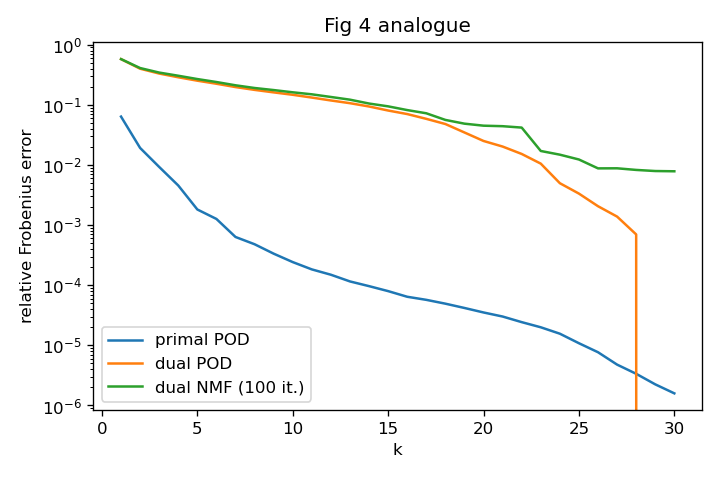
\includegraphics[width=0.7\linewidth]{figures/ch14r/hb_decay.png}
\caption{Best rank-$k$ approximation error of the 120 snapshots: primal POD, dual POD and dual NMF (100 iterations).}\label{fig:vf-hb-decay}
\end{figure}

\emph{Table~1 analogue.} At $\mu=(0.07,0.17)$, which is not in the snapshot set and where the full-order solve takes $1.9$~ms, \Cref{tab:vf-hb-t1} gives the comparison. The accuracy ordering matches the publication (the PB force error is much larger than the hybrid one at comparable displacement accuracy), but the speed-up is not reproduced: the hybrid model has 72 unknowns against 28 and its Lemke solve is slower than the full-order complementarity solve at 100 nodes.

\begin{table}[tbp]
\centering\footnotesize
\caption{Comparison at $\mu=(0.07,0.17)$.}\label{tab:vf-hb-t1}
\begin{tabular}{@{}lrrrr@{}}
\toprule
Model & Unknowns & Speed-up & Displacement error (\%) & Force error (\%)\\
\midrule
HR, $\epsilon_{\rm dual}=0.1$ & 72 & 0.64 (0.36 with reconstruction) & 0.48 & 14.1 on RID / 8.8 reconstructed\\
HR, 1 dual mode & 60 & 1.0 (0.29 with reconstruction) & 0.48 & 14.7 / 16.5\\
PB, $l_u=10$ & 20 & 3.8 & 0.22 & 38.4\\
PB, $l_u=14$ & 28 & 4.2 & 0.037 & 18.8\\
\emph{Publication: HR} & \emph{28} & \emph{8.5 / 5.9} & \emph{0.15} & \emph{13 / 12}\\
\emph{Publication: PB $l_u=9$} & \emph{18} & \emph{8.4} & \emph{0.32} & \emph{44}\\
\emph{Publication: PB $l_u=14$} & \emph{28} & \emph{9.1} & \emph{0.04} & \emph{23}\\
\bottomrule
\end{tabular}
\end{table}

\emph{Solutions and error over the parameter space.} \Cref{fig:vf-hb-sol} shows the displacement and the multipliers: the hybrid displacement cannot be told from the full-order one, the multipliers on the RID lie on the full-order values, and the reconstruction reproduces both contact zones with a slight overshoot at the second peak ($0.035$ against $0.033$); the PB models are accurate in displacement, but their multipliers oscillate and PB 9 overshoots the second peak by about $70\,\%$ ($0.056$ against $0.033$). Over the $100\times120$ test grid (\Cref{fig:vf-hb-errmap}, \Cref{tab:vf-hb-reg}) the displacement error has a mean of $0.74\,\%$ (publication $0.34\,\%$); the force errors are lower than the publication's, which is not a better method but a $2.5$ times larger RID (36 contacts against 14).

\begin{figure}[tbp]
\centering
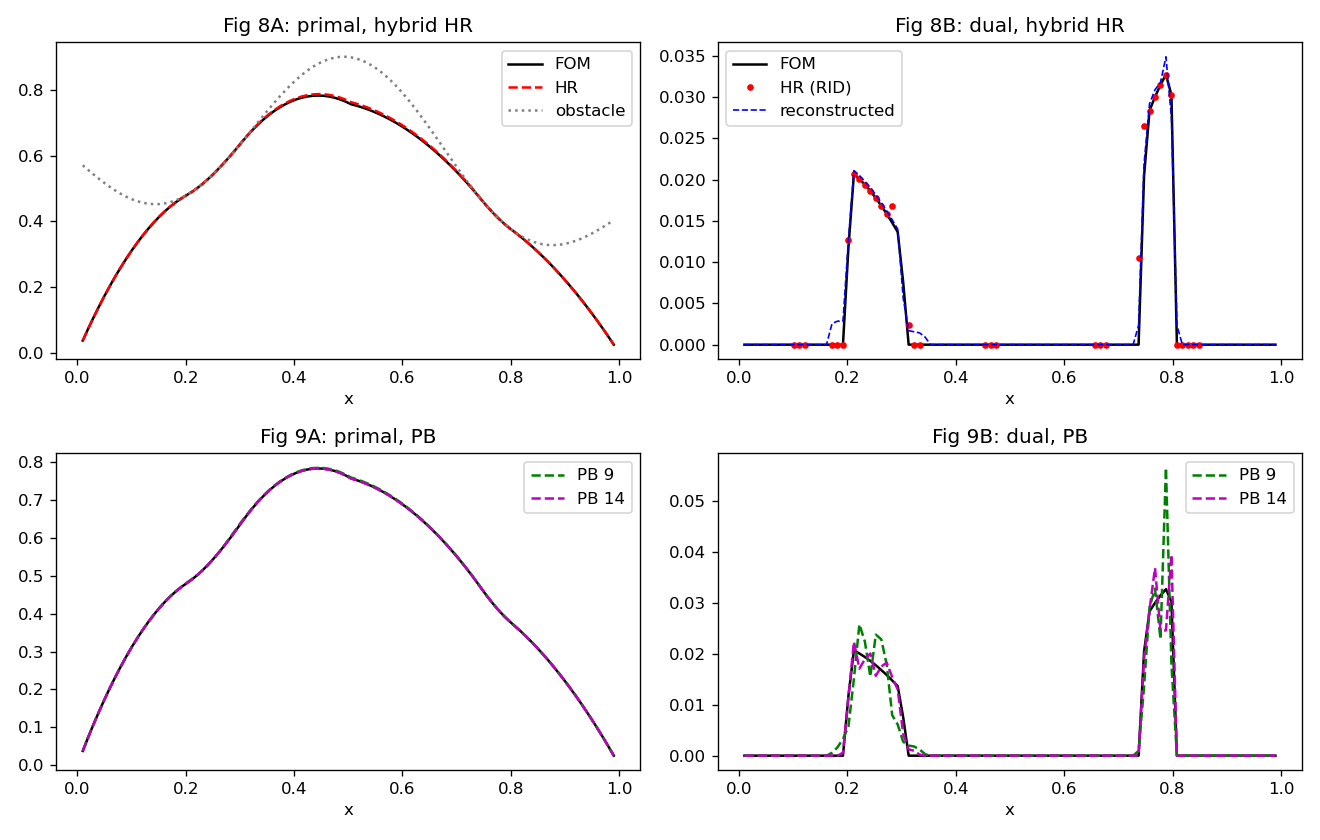
\includegraphics[width=0.95\linewidth]{figures/ch14r/hb_solutions.png}
\caption{Solutions at $\mu=(0.07,0.17)$: displacement (top left), multipliers of the full-order, the hybrid model on the RID and the reconstruction (top right), and the PB models with 9 and 14 modes (bottom).}\label{fig:vf-hb-sol}
\end{figure}

\begin{figure}[tbp]
\centering
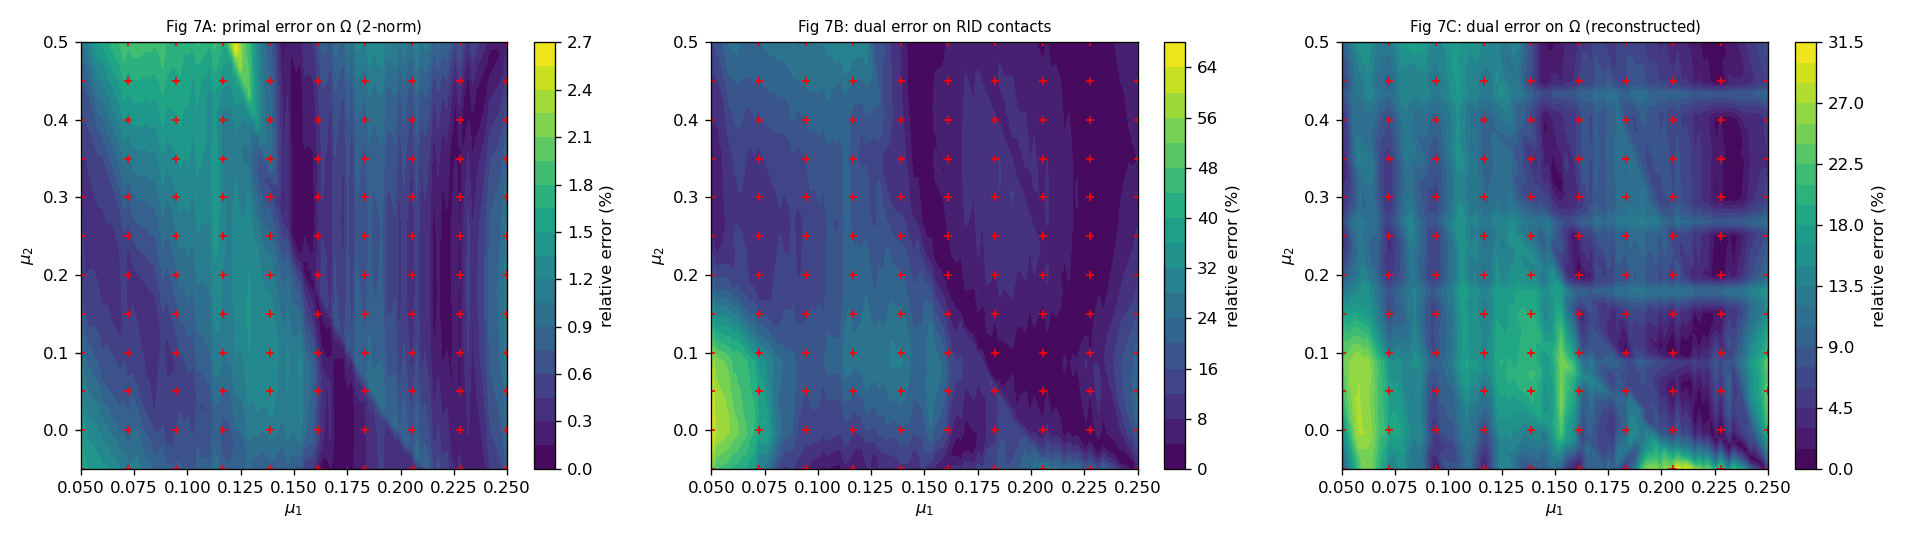
\includegraphics[width=0.98\linewidth]{figures/ch14r/hb_errmap_reg.png}
\caption{Error over the parameter space for the $10\times12$ snapshot grid, $100\times120$ test points: displacement (left), multipliers on the RID (centre), reconstructed multipliers (right); red crosses are the snapshots.}\label{fig:vf-hb-errmap}
\end{figure}

\begin{table}[tbp]
\centering\footnotesize
\caption{Error over the $100\times120$ test grid, regular snapshot grid (12\,000 parameter points, no Lemke failure).}\label{tab:vf-hb-reg}
\begin{tabular}{@{}lrrrr@{}}
\toprule
Quantity & Mean (\%) & Median (\%) & Max (\%) & Publication mean / max (\%)\\
\midrule
Displacement, 2-norm & 0.74 & 0.70 & 2.6 & 0.34 / 1.13\\
Contact force on RID & 13.1 & 10.8 & 66.6 & 24 / 148\\
Contact force over $\Omega$, reconstructed & 10.1 & 9.5 & 31.4 & 39 / 127\\
\bottomrule
\end{tabular}
\end{table}

\subsection*{Results: greedy sampling and the RID size}

With the greedy loop the first run (480 candidates, 50 iterations, $\epsilon_u=10^{-8}$, one element ring, contacts limited to nodes active in some snapshot $\pm1$ node) gives \Cref{fig:vf-hb-greedy1}: the hybrid force error on the RID falls to about $5\,\%$ and the reconstructed one to about $13\,\%$ while PB stays near $55\,\%$, which is the publication's main claim about contact forces; PB wins in the displacement 2-norm ($0.18\,\%$ against $0.49\,\%$) and in the $H^1$ norm the two end close together, so the claim that the hybrid model approximates gradients better is only weakly supported. The displacement accuracy was about $100$ times worse than the publication's ($0.49\,\%$ against $0.004\,\%$ mean).

\begin{figure}[tbp]
\centering
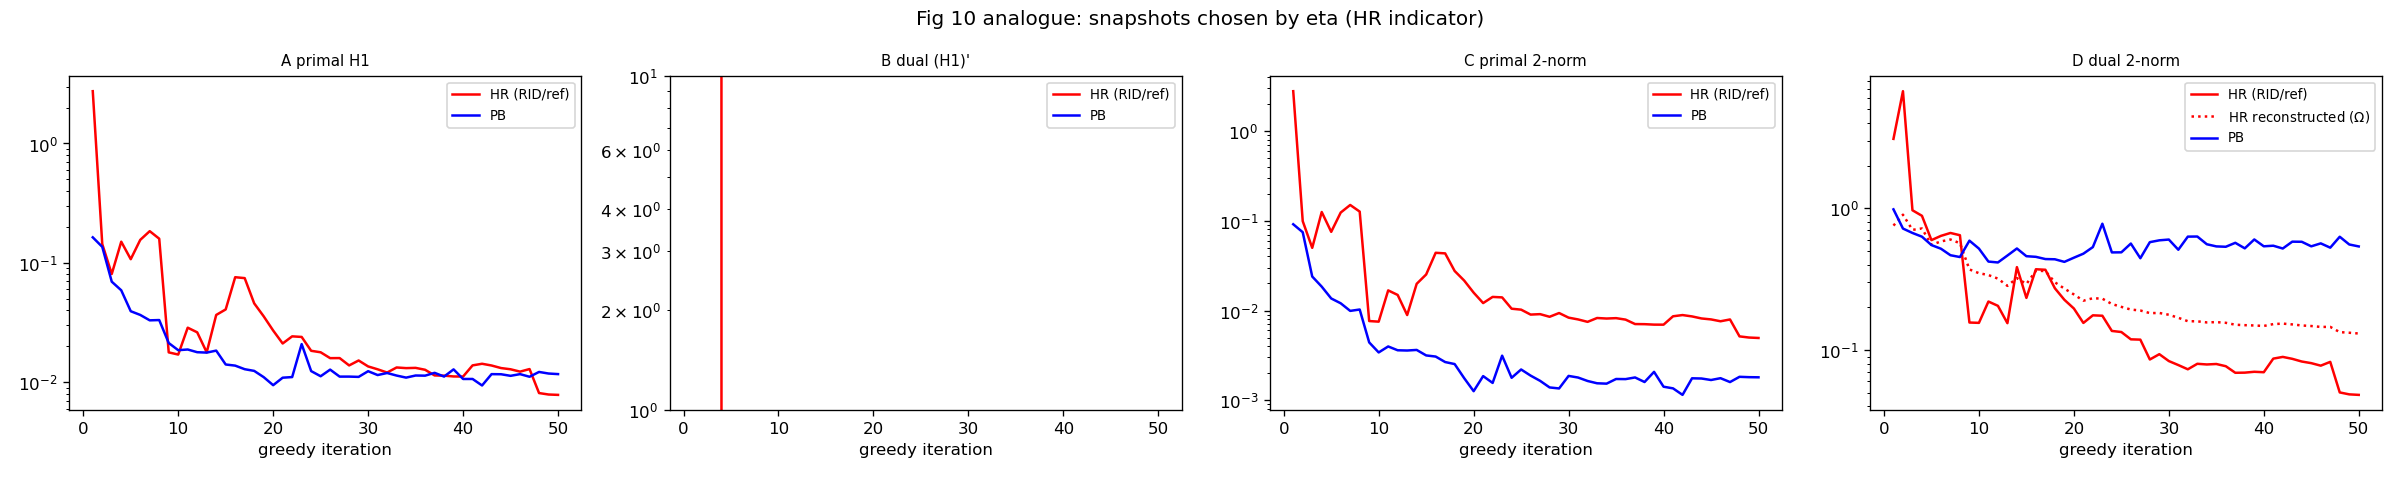
\includegraphics[width=0.95\linewidth]{figures/ch14r/hb_greedy_first.png}
\caption{Greedy loop driven by $\eta$, first run: average error over the 480 candidates for the hybrid (red; dotted: reconstructed multipliers) and PB (blue) models: (A) displacement, $H^1$; (B) multipliers, $(H^1)'$ (not usable in this run); (C) displacement, 2-norm; (D) multipliers, 2-norm.}\label{fig:vf-hb-greedy1}
\end{figure}

\emph{Two failure modes of the reduced system.} Both are properties of the formulation as stated and were diagnosed with scripts in the study. (1) If every node of $\mathcal P$ is a potential contact, the enriched basis has $|\mathcal P|$ columns, so $\mathbf A$ is square; for the $\eta$-selected set $|\mathcal P|=38$ with 38 columns, $\operatorname{cond}(\mathbf A)\approx10^{16}$, smallest singular value $3.7\times10^{-15}$ against $5.8\times10^1$, and the greedy runs gave displacement errors of $5$--$880\,\%$ and one ``good'' run ($0.0016\,\%$) that could not be reproduced. \Cref{tab:vf-hb-sing} lists the remedies tried; the one that works is to keep fewer potential contacts than $|\mathcal P|$, only the nodes that carried a contact force in some snapshot ($\pm1$ node), at the cost that contact outside the snapshot-observed zone is not enforced. (2) At the publication's $\epsilon_u=10^{-10}$ the loop showed spikes (error up to $32\,\%$); the Lemke solve failed on about $35\,\%$ of the parameters because the condensed matrix $\mathbf B_r\mathbf A^{-1}\mathbf B_r^{T}$ is strongly indefinite (minimum eigenvalue of its symmetric part about $-2\max|\text{entry}|$), and with the non-symmetric Petrov--Galerkin system nothing guarantees a well-posed complementarity problem. Alternatives (primal--dual active set, semismooth Newton) flagged $91$--$99\,\%$ of the cases as solved but had median errors of $2.7$--$6.3\,\%$; a symmetric Galerkin form on the RID is always well posed but about $10\,\%$ accurate. Coarsening to $\epsilon_u=10^{-8}$ (max error after iteration 20: $1.6\,\%$, final $0.49\,\%$) was the workaround of the first run.

\begin{table}[tbp]
\centering\footnotesize
\caption{Remedies for the singular reduced matrix ($\eta$-selected snapshots, 160 test parameters).}\label{tab:vf-hb-sing}
\begin{tabular}{@{}lrrrr@{}}
\toprule
Variant & RID nodes & $\operatorname{cond}(\mathbf A)$ & Displacement error median / max (\%) & Lemke failures\\
\midrule
Baseline (primal + dual DEIM, 1 ring) & 38 & $10^{16}$ & 0.36 / 4 & 0\\
+ DEIM on a stress basis & 54 & $2\times10^{16}$ & 6.4 / 73 & 16\\
+ stress DEIM, 2 rings & 72 & $4\times10^{16}$ & 6.4 / 86 & 28\\
+ stress DEIM, 3 rings & 88 of 98 & $6\times10^{3}$ & 0.002 / 0.02 & 0\\
\textbf{Potential contacts limited to ever-active nodes} & 38 & $\mathbf{7\times10^{6}}$ & 1.3 / 12 & 0\\
Same, plus 2 rings & 51 & $2\times10^{6}$ & 2.8 / 102 & 3\\
Unit-vector enrichment without orthogonalisation & 38 & $10^{16}$ & unchanged & ---\\
QR-whitening of the test space & 38 & $2\times10^{15}$ & unchanged & ---\\
Truncated pseudo-inverse of $\mathbf A$ & 38 & --- & about 99 & ---\\
\bottomrule
\end{tabular}
\end{table}

\emph{The remaining gap was the RID size.} A chain of negative results ruled out the other causes: the POD size (the Petrov--Galerkin system is square after enrichment, so the contact rows and not $l_u$ fix the accuracy), the dual mode count and the RID thickness at paper size, the indefiniteness of the complementarity matrix (a symmetric least-squares active-set solve was worse, $2.0\,\%$ mean, and giving it the exact full-order contact set still left $0.56$--$0.75\,\%$ error), the snapshot set (greedy snapshots were no better than 50 random ones) and the load sign (an exact mirror). Projecting the full-order solution on the enriched basis gives $0.004\,\%$ error, the publication's figure, while the hybrid solve gives $0.67\,\%$, so the basis was not the limit; the error enters when the displacements on $\mathcal P$ are tied to $\mathbf V\boldsymbol\gamma$, and the hybrid solve is no more accurate than interpolating the snapshot coefficients with no RID solve ($0.78\,\%$). What decides it is how much of the domain the RID covers (\Cref{fig:vf-hb-rid}): for 50 random snapshots a RID of 37 nodes gives $0.6\,\%$, 89 nodes $0.012\,\%$ (and $3\times10^{-4}\,\%$ with every RID node a contact and $\epsilon_u=10^{-10}$), 98 nodes exact; the dependence is not monotone below about 66 nodes, so a few extra rings are not enough unless the RID is large. The publication gives no final RID size.

\begin{figure}[tbp]
\centering
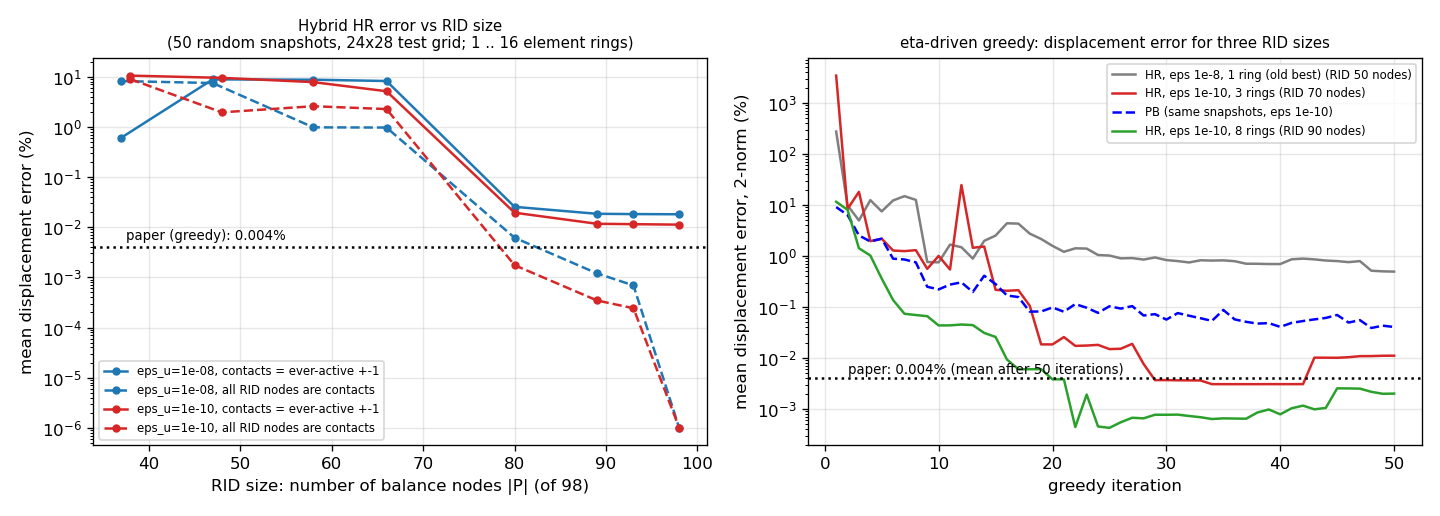
\includegraphics[width=0.98\linewidth]{figures/ch14r/hb_rid.png}
\caption{The RID size sets the accuracy. Left: mean displacement error of the hybrid model against the number of balance nodes $|\mathcal P|$ for RIDs grown by 1--16 rings, two POD tolerances and two contact sets; the dotted line is the publication's greedy accuracy. Right: mean error over the candidate set at each greedy iteration for three RID sizes; the blue dashed line is PB on the same snapshots.}\label{fig:vf-hb-rid}
\end{figure}

\Cref{tab:vf-hb-greedy} gives the greedy runs. With a large RID the $\epsilon_u=10^{-10}$ setting no longer needs the workaround, and the run `$\_$L3e10' (three rings, 70 nodes) is the closest match to the publication in all displacement and RID-force numbers (\Cref{fig:vf-hb-greedy2,fig:vf-hb-errmap2}); once the RID is large the hybrid model is 4 to 20 times more accurate than PB in displacement, and the larger RID also means no cost reduction on this 100-node mesh.

\begin{table}[tbp]
\centering\footnotesize
\setlength{\tabcolsep}{3pt}
\caption{Greedy runs (50 iterations, $\eta$-driven, 20$\times$24 candidates, $50\times60$ test grid).}\label{tab:vf-hb-greedy}
\begin{tabular}{@{}lrrrrrrr@{}}
\toprule
Run & $\epsilon_u$ & Rings & RID nodes & Unknowns & Displacement mean / max & Force on RID mean / max & Reconstructed mean / max\\
\midrule
first (\texttt{\_L1}) & $10^{-8}$ & 1 & 50 & 60 & 0.49\,\% / 3.1\,\% & 4.7\,\% / 66\,\% & 13\,\% / 66\,\%\\
\texttt{\_L8} & $10^{-8}$ & 8 & 90 & 66 & 0.025\,\% / 0.11\,\% & 12.6\,\% / 49.9\,\% & 14.4\,\% / 45.4\,\%\\
\texttt{\_L8e10} & $10^{-10}$ & 8 & 90 & 66 & 0.0021\,\% / 0.019\,\% & 0.25\,\% / 2.0\,\% & 8.0\,\% / 45.3\,\%\\
\texttt{\_L3e10} & $10^{-10}$ & 3 & 70 & 66 & 0.011\,\% / 0.084\,\% & 0.45\,\% / 9.6\,\% & 10.3\,\% / 36.1\,\%\\
Publication & $10^{-10}$ & --- & n/a & n/a & 0.004\,\% / 0.077\,\% & 0.34\,\% / 10\,\% & 1.3\,\% / 18\,\%\\
\bottomrule
\end{tabular}
\end{table}

\begin{figure}[tbp]
\centering
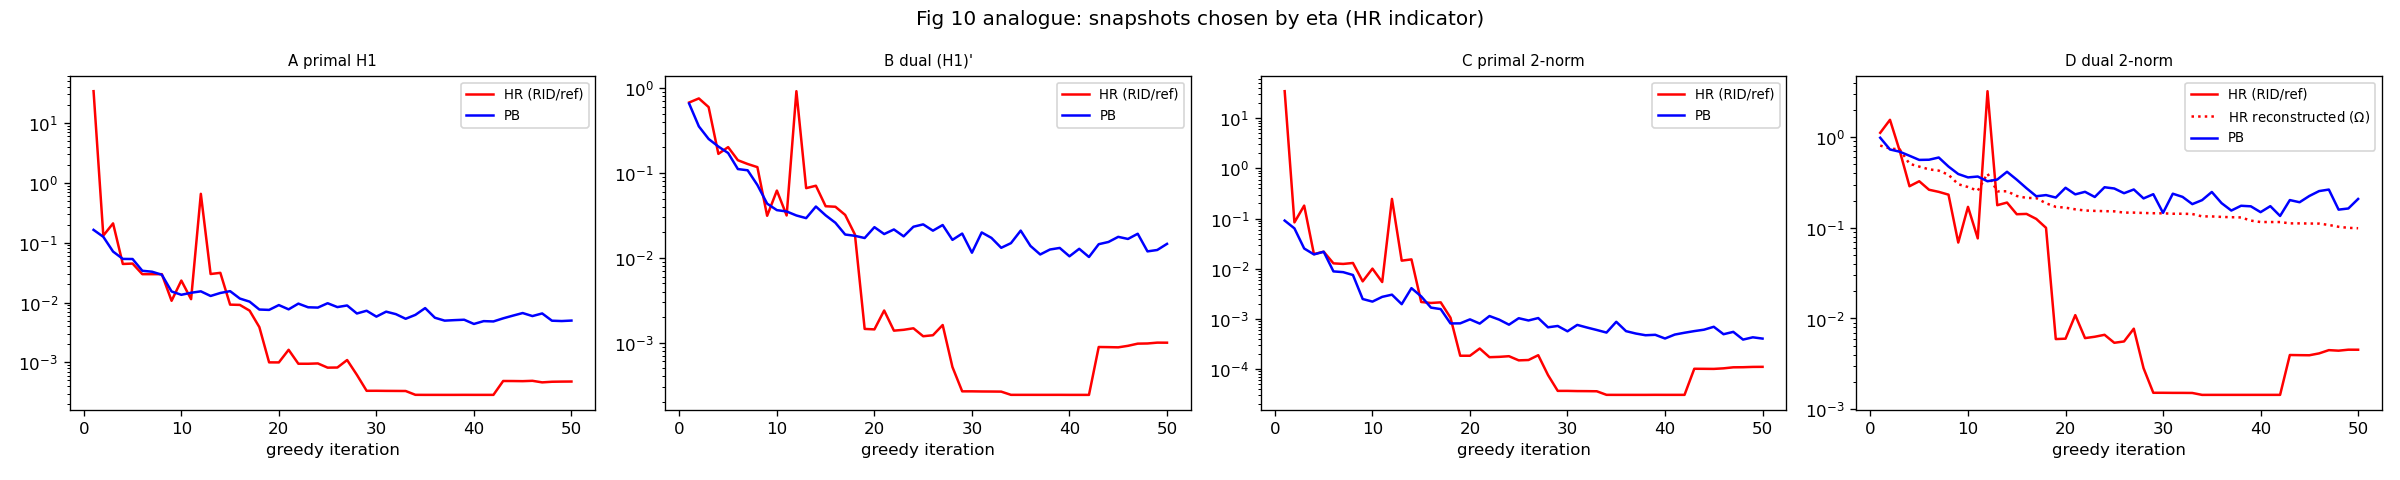
\includegraphics[width=0.95\linewidth]{figures/ch14r/hb_greedy_best.png}
\caption{Greedy loop driven by $\eta$, best run (3 rings, $\epsilon_u=10^{-10}$, 70 RID nodes), panels as in \Cref{fig:vf-hb-greedy1}. The hybrid displacement error falls to $3$--$5\times10^{-4}$ in the $H^1$ norm against $5\times10^{-3}$ for PB, with one spike at iteration 12 (a bad reduced complementarity solve).}\label{fig:vf-hb-greedy2}
\end{figure}

\begin{figure}[tbp]
\centering
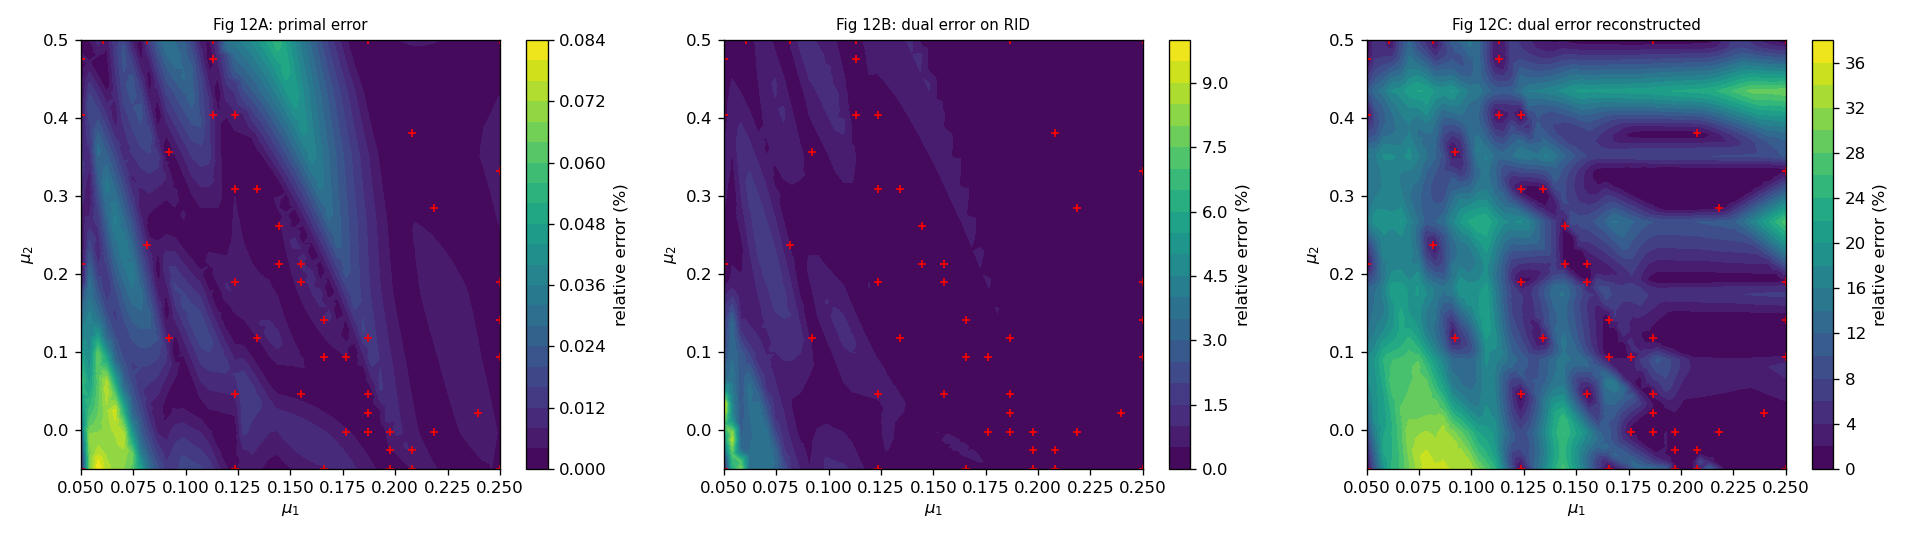
\includegraphics[width=0.95\linewidth]{figures/ch14r/hb_errmap_best.png}
\caption{Error maps after the greedy loop, best run, $100\times120$ test points: displacement (mean $0.011\,\%$, maximum $0.084\,\%$), multipliers on the RID (maximum about $10\,\%$) and reconstructed multipliers (maximum about $38\,\%$); highest at small $\mu_1$, where the contact zone is largest.}\label{fig:vf-hb-errmap2}
\end{figure}

\begin{figure}[tbp]
\centering
\includegraphics[width=1.0\linewidth]{figures/ch14_hyb.pdf}
\caption{Greedy loop for the rope problem of \citet{fauque2018hybrid}, best run. (a), (b) Error of the hybrid (HR, hyper-reduced) and projection-based (PB) reduced models against the iteration (displacement mean \cvfHybDispMean{}, maximum \cvfHybDispMax{}; contact force on the reduced domain \cvfHybForceMean{} mean, reconstructed force \cvfHybForceRecon{} mean at the end). (c) Size of the reduced problem.}\label{fig:vf-hyb}
\end{figure}

\subsection*{Geometry and mesh: the three-dimensional pellet--cladding problem}

One eighth of the problem is modelled, a $90^\circ$ sector and half the height, with symmetry planes $x=0$, $y=0$, $z=0$ (\Cref{fig:vf-hb3-geom}). The pellet has radius $R_p\le R_p^{\max}$, the cladding spans $4.1\le r\le4.7$~mm, and the half height is $6.75$~mm (the publication's pellet is 13.5~mm). The simulations S1--S5 differ only in the pellet radius: S1 $R_p=4.10$ (no gap), S2 $4.02$, S3 $4.06$, S4 $4.04$, S5 $4.08$. The loads are $5$~MPa axial on the pellet top and a radial pressure on the cladding outside of $250$~MPa for $z<2$~mm and $50$~MPa above, applied in 25 steps by a linear ramp. The material is $E=10^5$~MPa and $\nu=0.3$ for both bodies; the publication prints ``105 MPa'', which is read as $10^5$~MPa because with it the cladding closes by about $0.08$~mm at full load, which matches the gaps chosen in the publication. The mesh is a structured hexahedral mesh in $(r,\theta,z)$, pellet $6\times8\times27$ and cladding $3\times8\times27$ elements: 1944 elements, 2548 nodes, 6937 free degrees of freedom, with 252 node-to-node contact pairs on matching meshes and the axis nodes shared (collapsed hexahedra). The contact is frictionless and small-displacement with a gap along $\mathbf e_r$, $(\mathbf u_{\rm pellet}-\mathbf u_{\rm clad})\cdot\mathbf e_r\le4.1-R_p$, solved with the active-set solver of \fea{}. The RID is the union of the sets of displacement, stress and generalised-force modes (generalised forces being $\mathbf K\mathbf u$ over all degrees of freedom) and a region of interest (the top layer of the pellet and two element rings next to the axis, 16 elements; the publication does not specify it), extended by the contact-surface distance $d=0.1$~mm and one layer of elements.

\begin{figure}[tbp]
\centering
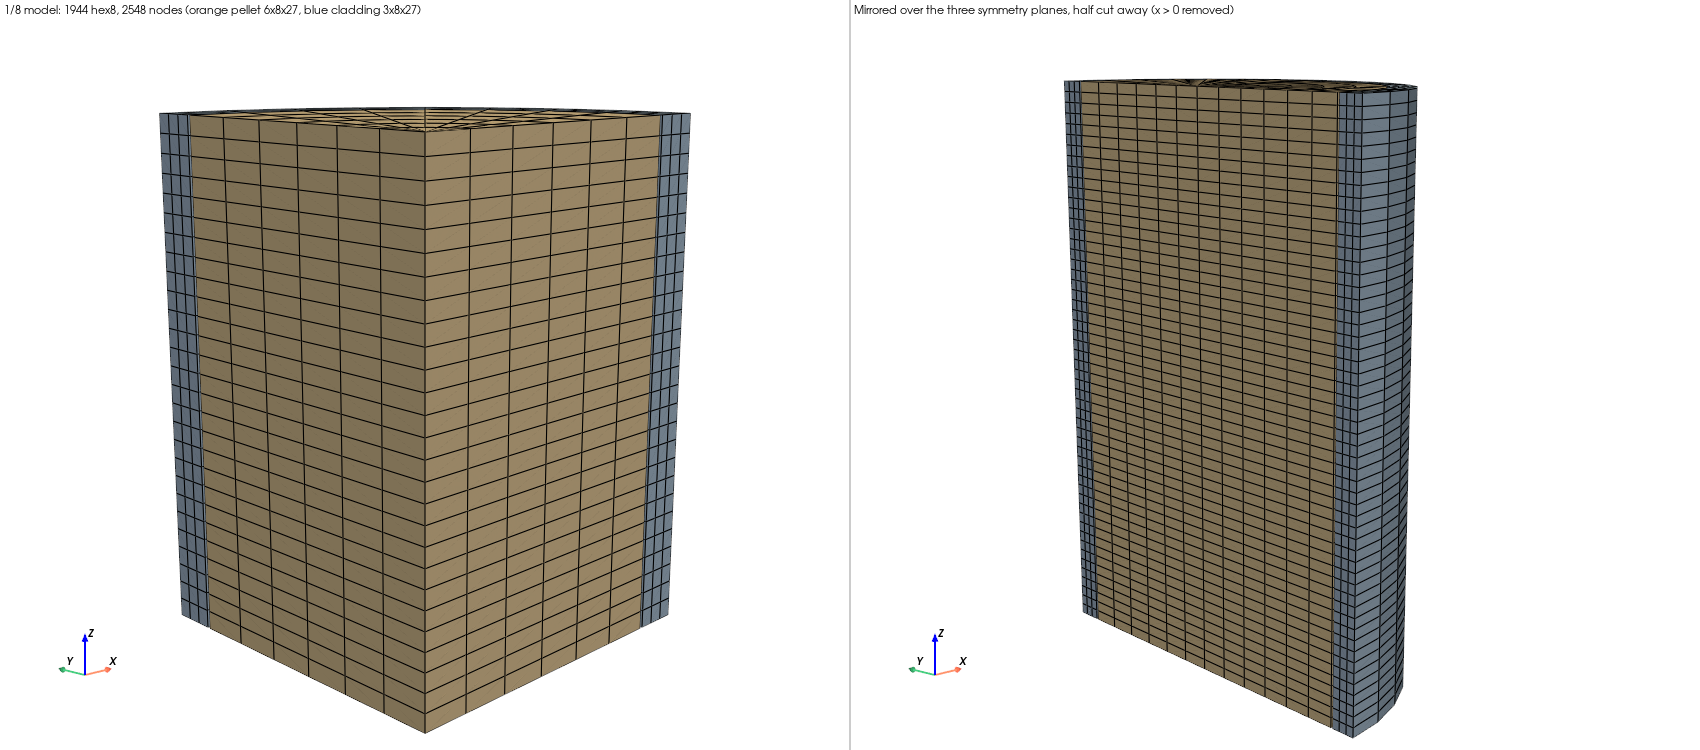
\includegraphics[width=0.95\linewidth]{figures/ch14r/hb3_geom.png}
\caption{Pellet--cladding model: the one-eighth model (pellet orange, cladding blue, case S3) and the same mesh mirrored over the symmetry planes with one half cut away.}\label{fig:vf-hb3-geom}
\end{figure}

\emph{Validation of the finite element model.} Rigid translations lie in the null space of the unconstrained stiffness (residual $10^{-15}$); the Lam\'e thick cylinder under external pressure, with three elements through the thickness, gives inner and outer radial displacements within $0.25\,\%$ and $0.23\,\%$ of the closed form (angular spread $2\times10^{-14}$); and pellet uniaxial compression gives the exact top displacement and $\sigma_{zz}=-5$~MPa in every element. An earlier version used the transposed Jacobian inverse (errors of $17$--$69\,\%$ in the Lam\'e test), fixed and verified by these checks. The full-order behaviour: S1 has all 252 pairs in contact from step 1; S2 first touches at step 25 (18 pairs); S3 at step about 12 (63 pairs at the end); S4 at about step 16 (36 pairs); S5 at about step 6 (90 pairs). \Cref{fig:vf-hb3-fom} shows the stresses of S3: the cladding is pressed in by up to $0.044$~mm where the 250~MPa pressure acts and has closed the gap there, its hoop stress reaches about $-1000$~MPa (von Mises up to $1062$~MPa) while the pellet stays below about $250$~MPa, with a stress concentration at the end of the contact zone ($z\approx1.5$--$2$~mm).

\begin{figure}[tbp]
\centering
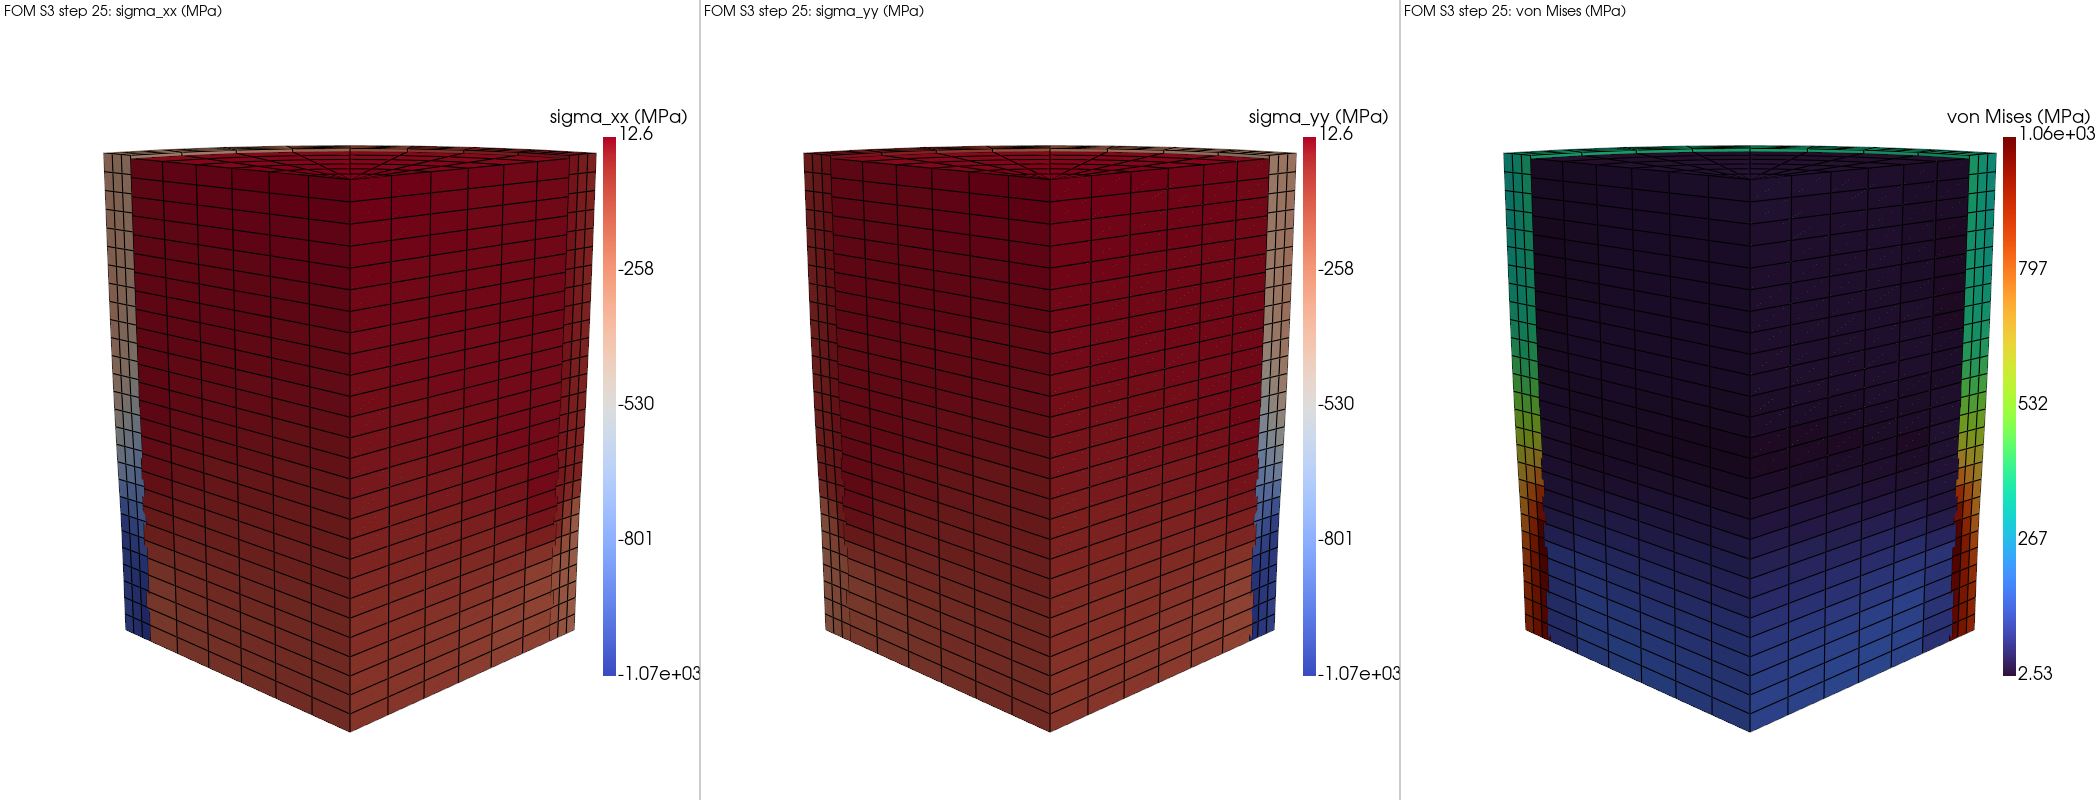
\includegraphics[width=0.95\linewidth]{figures/ch14r/hb3_fom.png}
\caption{Full-order solution of S3 at step 25 (deformation magnified three times, element-centroid values): $\sigma_{xx}$, $\sigma_{yy}$ and von Mises stress seen from the symmetry planes.}\label{fig:vf-hb3-fom}
\end{figure}

\subsection*{Results: prediction of S3 from snapshots}

The error of the displacement is the maximum over RID degrees of freedom of $|\mathbf u_{HR}-\mathbf u_{FOM}|/\max|\mathbf u_{FOM}|$ at the worst step, that of the stress the same for $\sigma_{11}$ over RID elements, and ``agree'' is the fraction of RID contact pairs whose active or inactive state matches the full-order one at the worst step (publication: displacement $1\,\%$, stress $5\,\%$, speed-up $10$). \Cref{tab:vf-hb3-cases} and \Cref{fig:vf-hb3-err} give the cases. With the publication's training set (S1 and S2, case A) the error reaches $13$--$19\,\%$ in displacement; adding two simulations with intermediate gaps (S4, S5, case B, which interpolates in the gap and never uses S3) reduces it to $0.05\,\%$ in displacement and $0.21\,\%$ in stress with a correct contact set at every step (B2), better than the publication's limits. Before contact starts (steps 1--11) all cases are accurate to $0.26\,\%$ or better, and the error of every case changes at contact onset (step 12). Timings come from single runs and vary by about $\pm20\,\%$.

\begin{table}[tbp]
\centering\footnotesize
\setlength{\tabcolsep}{3pt}
\caption{Prediction of S3 (25 steps). Modes u/s/F: displacement, stress, generalised-force modes.}\label{tab:vf-hb3-cases}
\begin{tabular}{@{}llrrrrrrrr@{}}
\toprule
Case & Training & POD tol. & Modes u/s/F & RID elements & Contact pairs & Disp. & Stress & Agree & Speed-up\\
\midrule
A1 & S1+S2 (publication), minimal enrichment & $10^{-5}$ & 3/3/3 & 12\,\% & 42 & 19.3\,\% & 8.8\,\% & 71\,\% & 9.6$\times$\\
A2 & S1+S2, full FE contact dofs, 2 layers & $10^{-11}$ & 4/4/4 & 26\,\% & 73 & 13.4\,\% & 10.0\,\% & 88\,\% & 5.7$\times$\\
B1 & S1+S2+S4+S5, full FE contact dofs & $10^{-5}$ & 4/6/11 & 29\,\% & 130 & 3.35\,\% & 4.04\,\% & 93\,\% & 4.0$\times$\\
\textbf{B2} & same, 1 layer & $10^{-8}$ & 9/12/12 & 32\,\% & 142 & \textbf{0.050\,\%} & \textbf{0.21\,\%} & 100\,\% & 3.7$\times$\\
B3 & same, 1 layer & $10^{-11}$ & 13/14/15 & 33\,\% & 148 & 0.055\,\% & 0.055\,\% & 100\,\% & 3.5$\times$\\
B4 & same, 2 layers & $10^{-11}$ & 13/14/15 & 59\,\% & 190 & 0.010\,\% & 0.017\,\% & 100\,\% & 2.1$\times$\\
Publication & S1+S2 & $10^{-5}$ & 17/20/21 & --- & --- & 1\,\% & 5\,\% & --- & 10$\times$\\
\bottomrule
\end{tabular}
\end{table}

\begin{figure}[tbp]
\centering
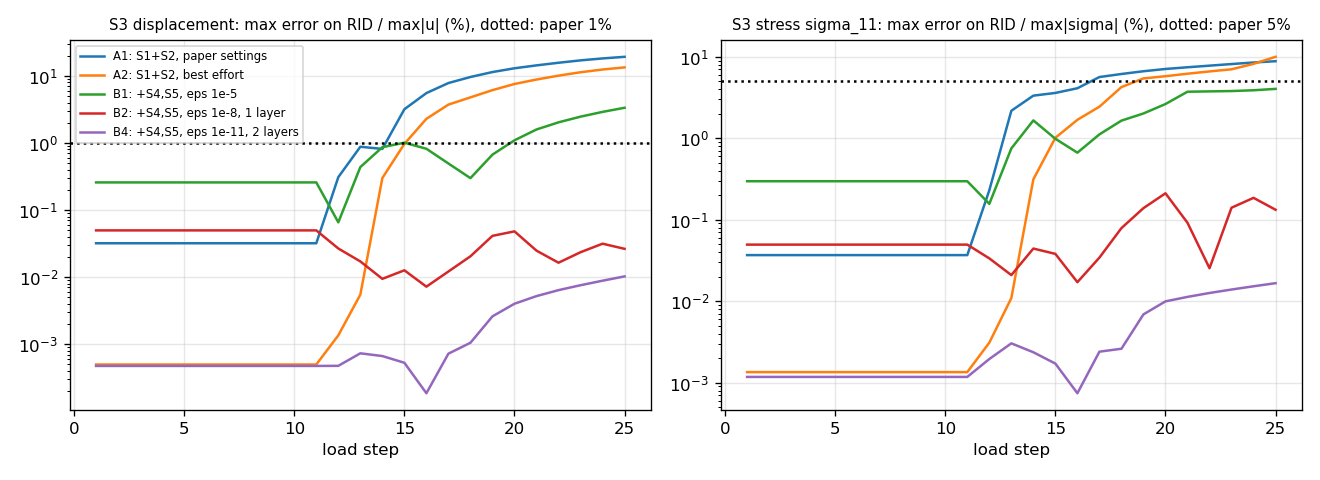
\includegraphics[width=0.95\linewidth]{figures/ch14r/hb3_errors.png}
\caption{Prediction error of S3 at each load step for cases A1--B4: displacement (left) and $\sigma_{11}$ (right), maximum over the RID relative to the maximum value; dotted lines are the publication's $1\,\%$ and $5\,\%$.}\label{fig:vf-hb3-err}
\end{figure}

\emph{Why the publication's training set is not enough here.} The 50 snapshots of S1 and S2 have normalised singular values $1$, $0.11$, $5.6\times10^{-3}$, $5.2\times10^{-5}$ and then $10^{-15}$: rank 4. S1 is bonded and exactly linear in the load, and S2 is free until the last step. A POD tolerance of $10^{-5}$ gives 3 modes, not the publication's 17, and the four-mode basis alone has a $6\,\%$ projection error on the last step of S3 (\Cref{fig:vf-hb3-rank}); S3's contact reaction is up to $61\,\%$ of its solution but only one S2 step (18 pairs) shows contact in the training data. The publication's 17, 20 and 21 modes mean its S1 and S2 snapshots contained much richer contact evolution; why could not be recovered. Adding S4 and S5 gives a slowly decaying spectrum and 9 modes at tolerance $10^{-8}$, with the projection error of S3 below $5\times10^{-4}$ at every step. A second finding is that keeping every primal degree of freedom of the potential contact zone as a finite element degree of freedom (the publication's Sec.~7.3) is essential: with the minimal rank-completing enrichment of the rope case and the same training data the error is $13.7\,\%$ against $3.35\,\%$ (B1).

\begin{figure}[tbp]
\centering
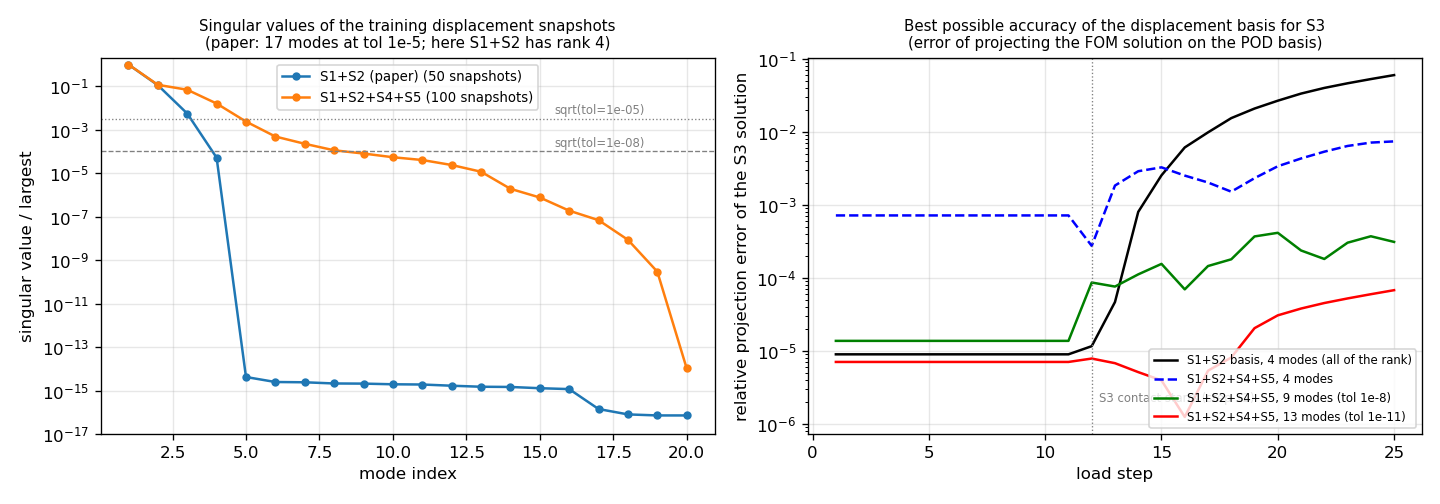
\includegraphics[width=0.95\linewidth]{figures/ch14r/hb3_rank.png}
\caption{Left: singular values of the displacement snapshots for S1+S2 (50 snapshots, exactly four non-negligible values) and S1+S2+S4+S5 (100). Right: projection error of the full-order S3 solution on the basis, the best any model built on it can do.}\label{fig:vf-hb3-rank}
\end{figure}

\emph{Fields, RID and contact.} \Cref{fig:vf-hb3-hrom} compares the von Mises stress of the full model and of case B2 on the whole body: the fields are visually identical and the largest difference is $1.05$~MPa against a peak of $1062$~MPa ($0.10\,\%$); the displacement magnitude differs by a relative $L^2$ error of $4.0\times10^{-4}$. \Cref{fig:vf-hb3-rid} shows the RID, 616 of 1944 elements ($32\,\%$), and the contact force per pair, active only below $z=2$~mm. The contact behaviour of S1--S3 is in \Cref{fig:vf-hb3-contact}: S1 is in contact everywhere with the largest forces below $z=2$~mm, S2 has only just touched (18 pairs), S3 has 63 active pairs for $z<1.5$~mm, which is why S1 and S2 alone teach the basis almost nothing about partial contact; the loaded zone grows upwards with the load, the peak is about 16~N per pair, and the cladding moves in by about 44~\textmu m at the bottom while the pellet moves about 4~\textmu m, so the difference of 40~\textmu m equals the initial gap where the surfaces touch; the HROM markers lie on the full-order curves.

\begin{figure}[tbp]
\centering
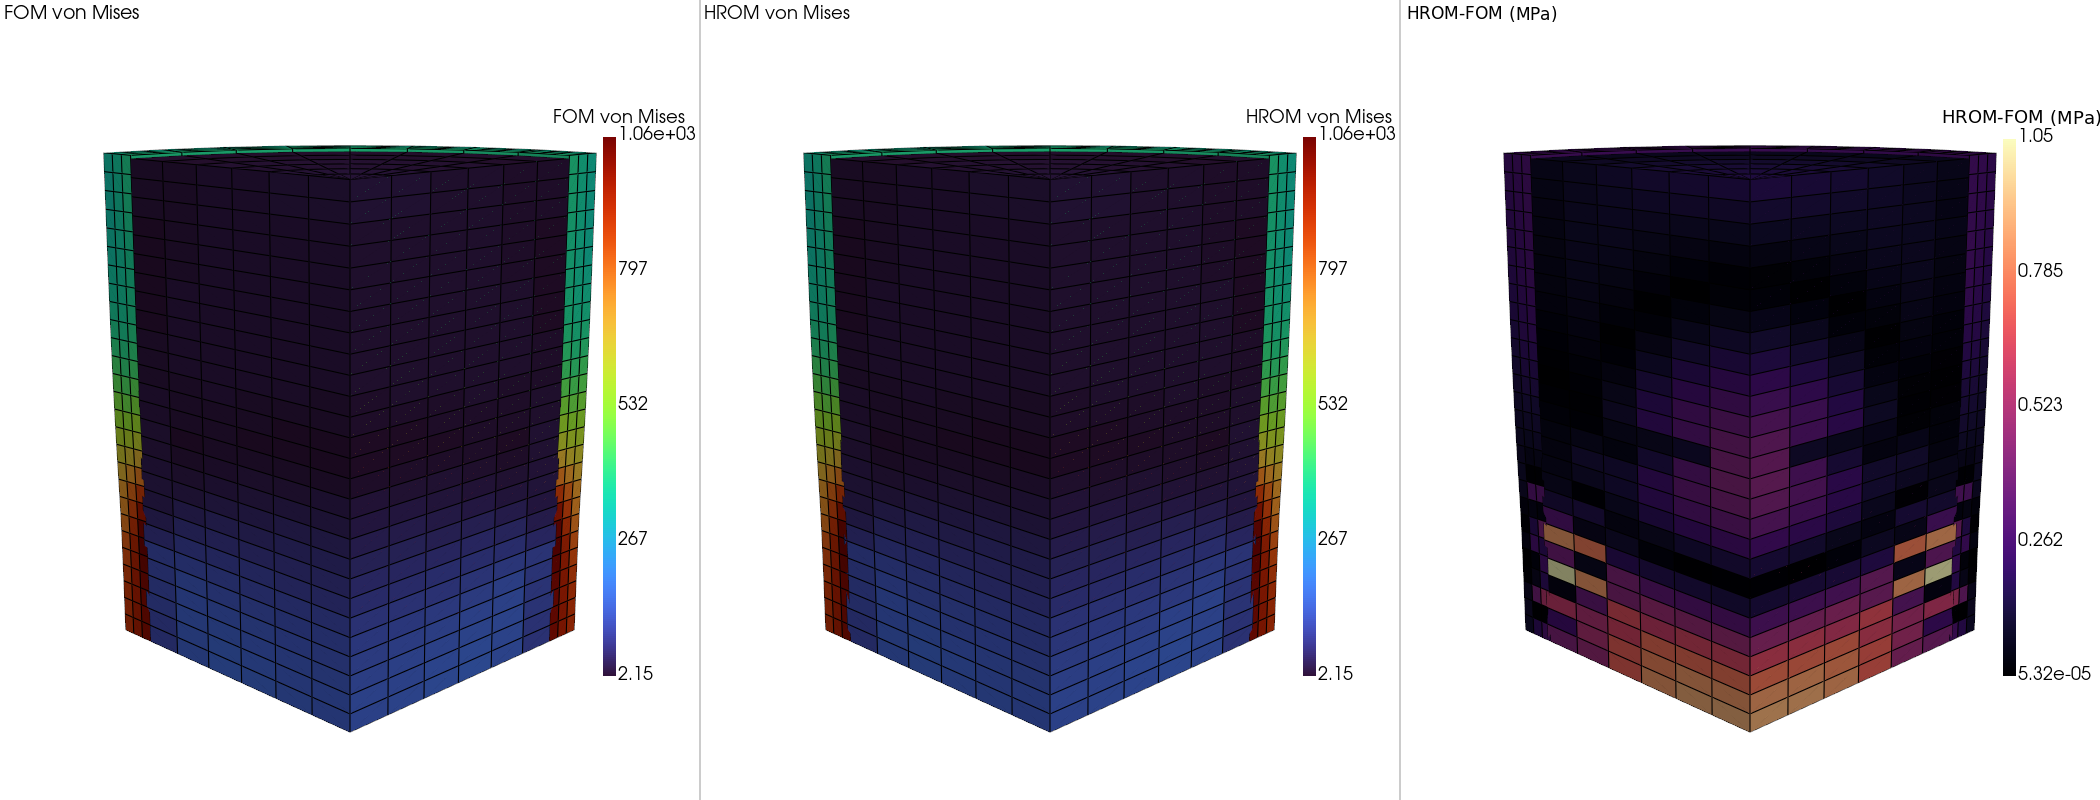
\includegraphics[width=0.98\linewidth]{figures/ch14r/hb3_hrom.png}
\caption{Hybrid HROM against the full model for S3 at step 25 (case B2): von Mises stress from the full model, from the HROM reconstructed on the whole body, and their absolute difference.}\label{fig:vf-hb3-hrom}
\end{figure}

\begin{figure}[tbp]
\centering
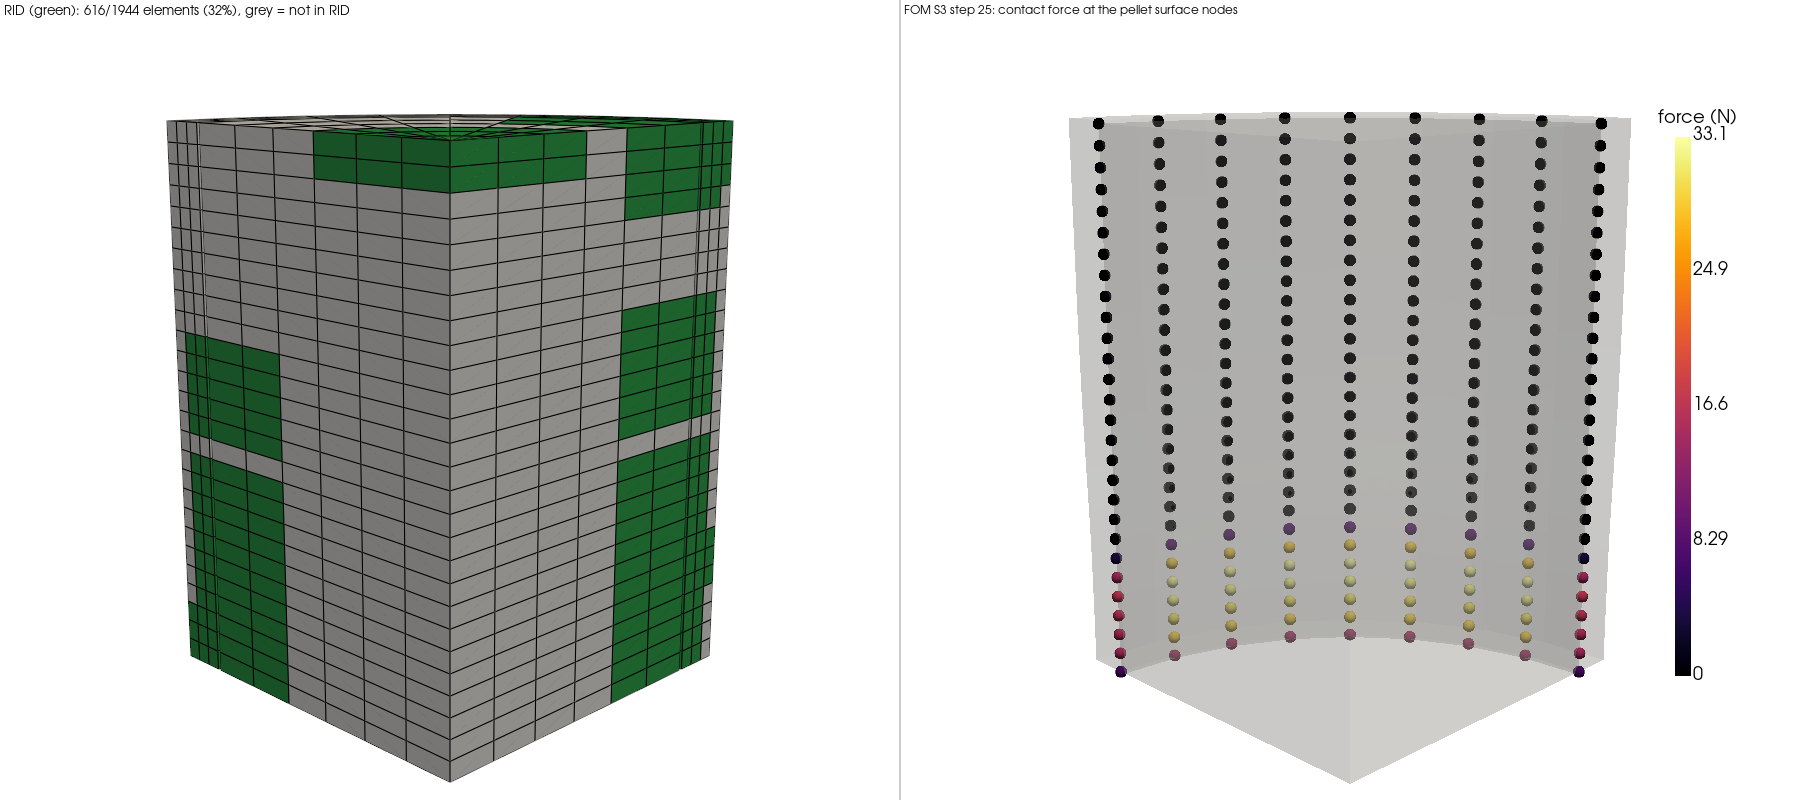
\includegraphics[width=0.95\linewidth]{figures/ch14r/hb3_rid.png}
\caption{Left: the RID (616 of 1944 elements, green). Right: contact force per pair on the pellet surface nodes at step 25.}\label{fig:vf-hb3-rid}
\end{figure}

\begin{figure}[tbp]
\centering
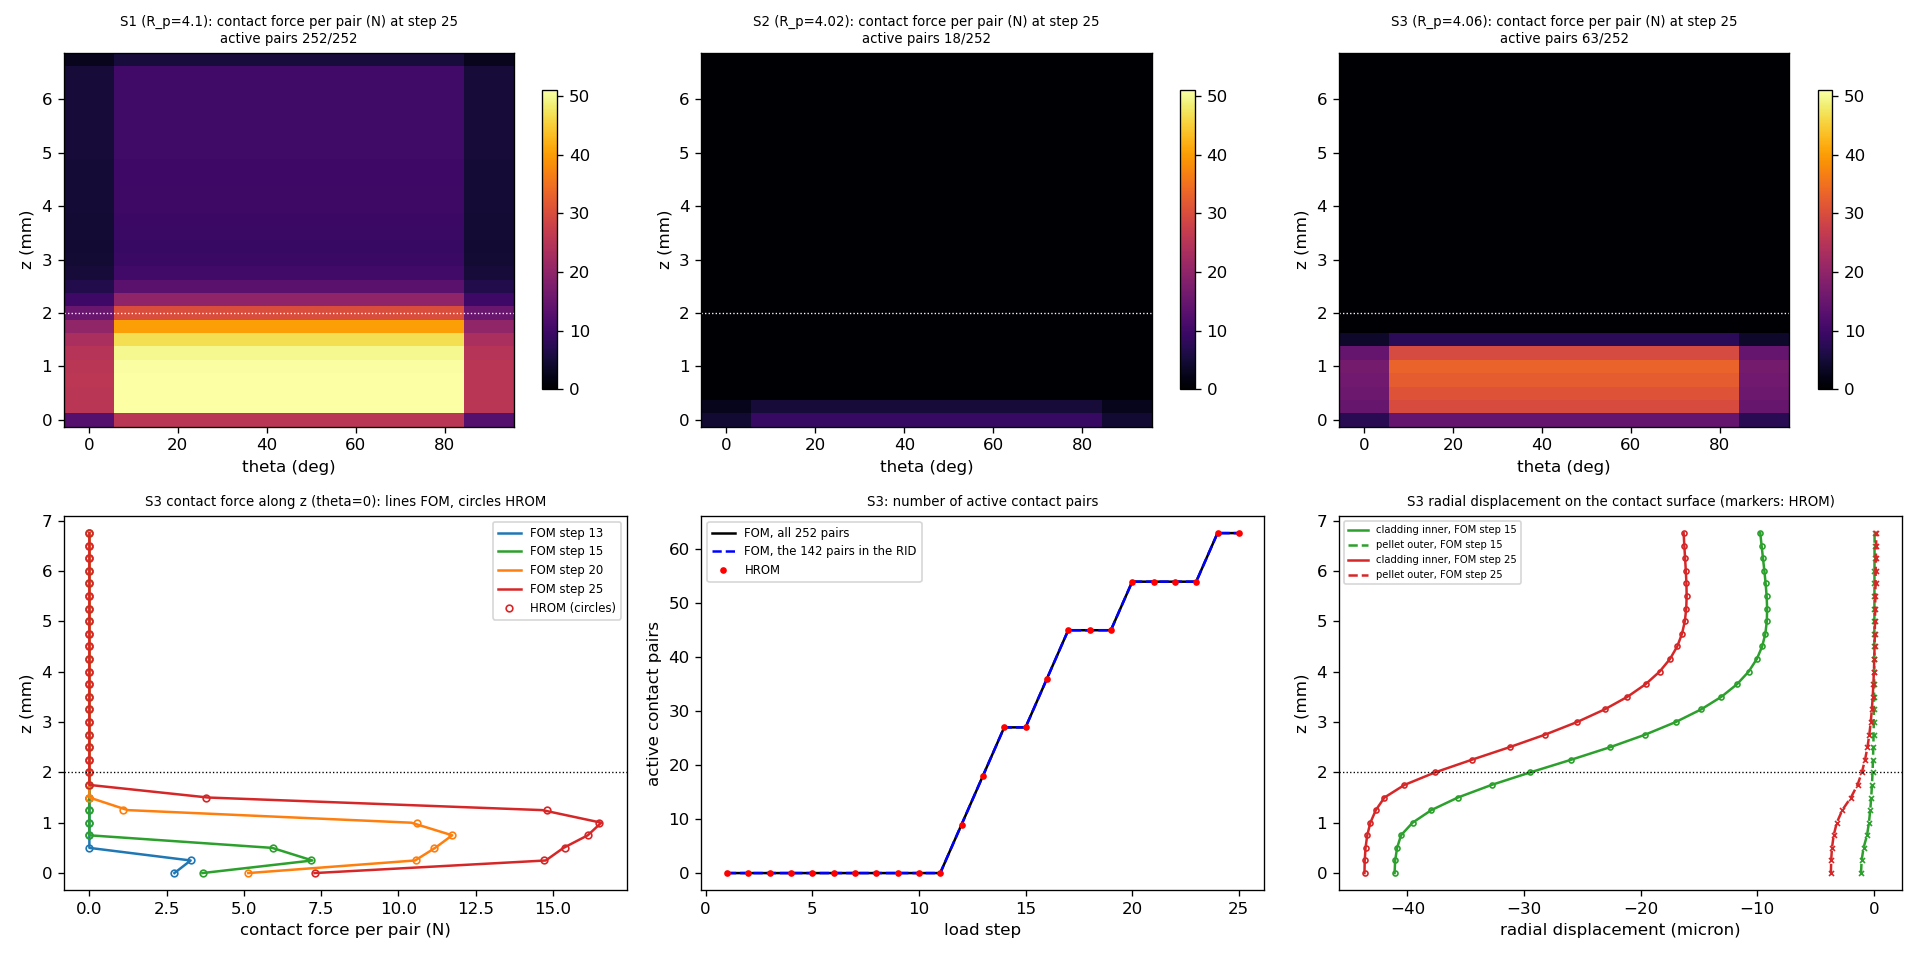
\includegraphics[width=0.98\linewidth]{figures/ch14r/hb3_contact.png}
\caption{Contact behaviour: contact force per pair over the contact surface for S1, S2, S3 (top); S3 contact force along $z$ at several steps, number of active pairs per step for the full model, the restricted count and the HROM, and radial displacements of the cladding inner surface and of the pellet outer surface (bottom).}\label{fig:vf-hb3-contact}
\end{figure}

\subsection*{Results: mesh refinement, RID size and extrapolation (3D)}

The case B2 model was run on meshes refined in all directions (\Cref{tab:vf-hb3-mesh}, \Cref{fig:vf-hb3-mesh}). The full-order time grows about 24 times for 7.3 times more degrees of freedom (sparse LU and the dense Delassus matrix with one column per contact pair), while the HROM time grows only 1.5 times, because the RID barely grows (616 to 914 elements); the speed-up therefore rises from $3.2$ to $11$ to $50$, and the publication's $10\times$ is crossed between the first two meshes. The low speed-up of the baseline is a consequence of the small mesh and not of the method, but the speed-up at the publication's mesh size cannot be stated because its mesh size is not given. Accuracy stays inside the publication's limits on all three meshes (displacement below $0.23\,\%$, $\sigma_{11}$ below $1.3\,\%$), a factor of 4 to 6 larger than on the baseline, and the contact-force error rises from $1.9\,\%$ to $7$--$8\,\%$. A caveat is that on the refined meshes the RID rows contain only 104 of the 221 contact pairs active for S3 at the last step, and the contact-set agreement inside the RID drops to $95.8\,\%$; the pairs outside the RID are not enforced, yet the errors stay small, and where those pairs lie was not examined. The offline time grows from 19~s to 140~s.

\begin{table}[tbp]
\centering\footnotesize
\setlength{\tabcolsep}{3pt}
\caption{Mesh study (case B2; S3 prediction). Meshes: elements per direction (pellet radial, cladding radial, circumferential, axial).}\label{tab:vf-hb3-mesh}
\begin{tabular}{@{}lrrrrrrrr@{}}
\toprule
Mesh & Elements & Free dofs & Contact pairs & RID elements & FOM time (s) & HROM time (s) & Speed-up & Worst $u$ / $\sigma_{11}$ / force error\\
\midrule
L1 (6, 3, 8, 27) & 1944 & 6937 & 252 & 616 (31.7\,\%) & 5.6 & 1.76 & 3.2$\times$ & 0.050 / 0.21 / 1.9\,\%\\
L1.5 (9, 5, 12, 40) & 6720 & 22\,600 & 533 & 860 (12.8\,\%) & 23.2 & 2.10 & 11.0$\times$ & 0.18 / 1.21 / 7.5\,\%\\
L2 (12, 6, 16, 54) & 15\,552 & 50\,936 & 935 & 914 (5.9\,\%) & 134.9 & 2.71 & 49.7$\times$ & 0.23 / 1.27 / 8.4\,\%\\
\bottomrule
\end{tabular}
\end{table}

\begin{figure}[tbp]
\centering
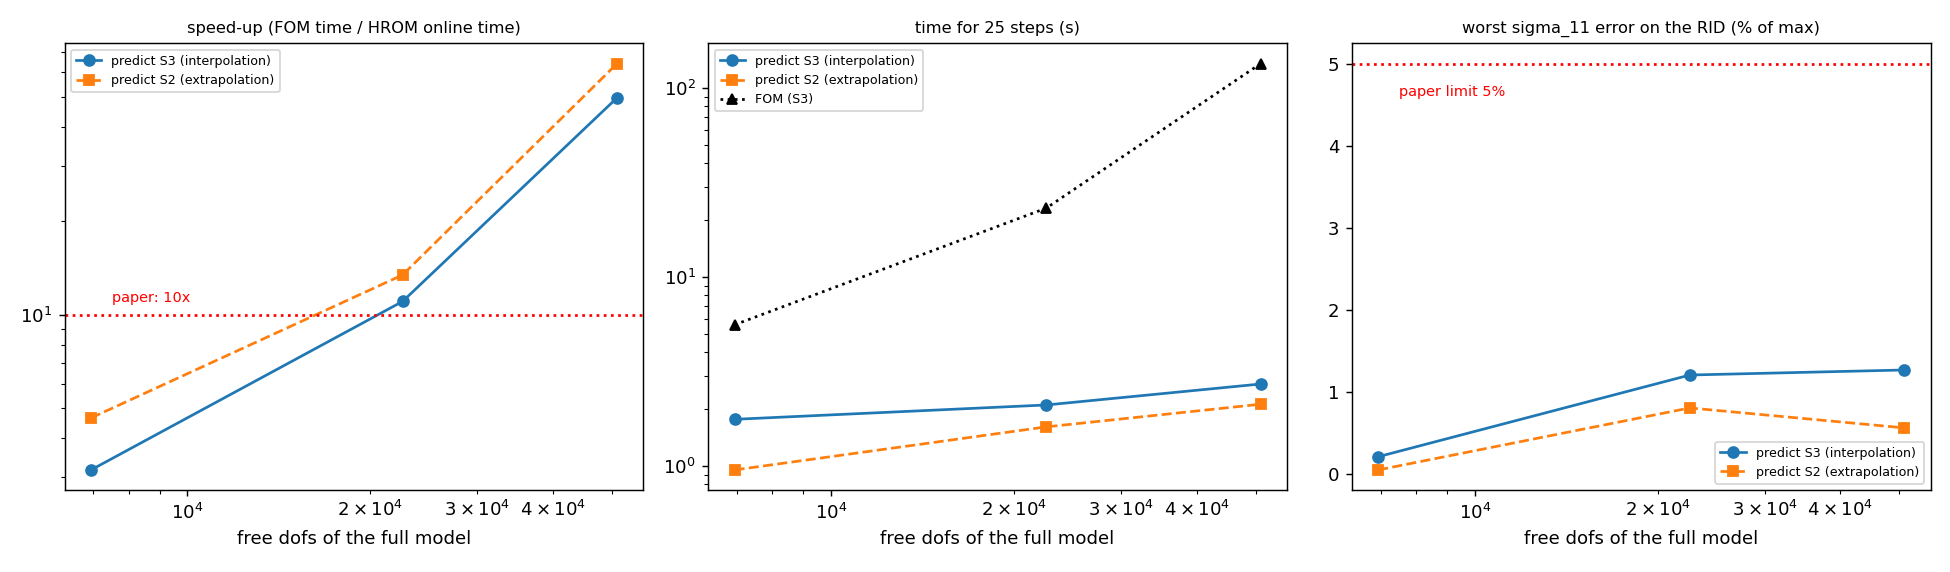
\includegraphics[width=0.95\linewidth]{figures/ch14r/hb3_mesh.png}
\caption{Mesh study: speed-up, computing time and worst $\sigma_{11}$ error against the number of free degrees of freedom, for S3 (solid) and the extrapolation case S2 (dashed); the red dotted lines are the publication's $10\times$ and $5\,\%$.}\label{fig:vf-hb3-mesh}
\end{figure}

A larger RID (two rings, or $d=0.3$~mm) covers more of the active pairs (130 of 221 with two layers on L2) but does not improve the errors usefully: displacement and stress errors change by less than $0.05$ percentage points, the force error stays at $7$--$9\,\%$ and the speed-up falls by half (L2: $49.7\times$ to $22.5\times$); the single-layer RID with $d=0.1$~mm remains the best trade-off. To test an edge case, S2 (the smallest radius, the largest gap) was predicted from S1, S3, S4, S5, so it lies outside the training range (\Cref{tab:vf-hb3-extra}); the case S6 ($R_p=3.98$~mm) never touches and is not a contact test.

\begin{table}[tbp]
\centering\footnotesize
\caption{Extrapolation to S2 ($R_p=4.02$ mm) from S1, S3, S4, S5.}\label{tab:vf-hb3-extra}
\begin{tabular}{@{}lrrrrrrr@{}}
\toprule
Mesh & RID elements & S2-active pairs in RID & Speed-up & Worst $u$ & Worst $\sigma_{11}$ & Worst force & Min.\ agreement\\
\midrule
L1 & 617 & 18/18 & 4.7$\times$ & 0.029\,\% & 0.050\,\% & 1.9\,\% & 100\,\%\\
L1.5 & 854 & 26/26 & 13.4$\times$ & 0.66\,\% & 0.81\,\% & 25.6\,\% & 92.7\,\%\\
L2 & 902 & 27/51 & 64.0$\times$ & 0.24\,\% & 0.56\,\% & 16.3\,\% & 100\,\%\\
\bottomrule
\end{tabular}
\end{table}

\subsection*{Comparison with the publication}

\begin{table}[tbp]
\centering\footnotesize
\caption{Outcome of the reproduction of \citet{fauque2018hybrid}.}\label{tab:vf-hb-cmp}
\begin{tabularx}{\linewidth}{@{}>{\raggedright\arraybackslash}p{4.3cm} >{\raggedright\arraybackslash}X >{\raggedright\arraybackslash}p{2.4cm}@{}}
\toprule
Result & This work & Outcome\\
\midrule
Rope, regular grid: displacement error (mean / max) & $0.74\,\%$ / $2.6\,\%$ against $0.34\,\%$ / $1.13\,\%$ & about 2$\times$ worse\\
Rope, regular grid: forces & $13\,\%$ / $67\,\%$ on RID with a $2.5\times$ larger RID; same HR-below-PB ordering & reproduced (ordering)\\
Rope, greedy: displacement error & $0.011\,\%$ / $0.084\,\%$ against $0.004\,\%$ / $0.077\,\%$ (RID of 70 nodes) & reproduced\\
Rope, greedy: force on RID & $0.45\,\%$ / $9.6\,\%$ against $0.34\,\%$ / $10\,\%$ & reproduced\\
Rope, greedy: reconstructed force & $10.3\,\%$ / $36\,\%$ against $1.3\,\%$ / $18\,\%$ & not reproduced\\
HR more accurate than PB in $H^1$ & yes with a large RID, weak with a small one & reproduced (large RID)\\
Rope speed-up & $0.6$--$1\times$ against $8.5\times$ & not reproduced\\
3D, publication's training set (S1+S2) & $13$--$19\,\%$ displacement error against $1\,\%$ & not reproduced\\
3D, with S4, S5 added & $0.05\,\%$ / $0.21\,\%$, correct contact set & reproduced, training set changed\\
3D speed-up & $3.7\times$ on the baseline mesh, $11\times$ and $50\times$ refined, against $10\times$ & partly\\
\bottomrule
\end{tabularx}
\end{table}

\subsection*{Open details and the speed-ups}

The publication leaves open several details that decide the numbers (\Cref{tab:vf-hb-gaps}); the final RID size and the contact-node set should be treated as free tuning parameters unless the authors' code is available. The speed-up on the rope is not reproduced because with a 70--90 node RID on a 100-node mesh there is little to gain, and the three-dimensional speed-up depends on a mesh size the publication does not state. The 4 against 1 dual mode count was not resolved, the reconstruction of forces outside the RID (\cref{eq:hb-nnls}) is worse than the publication's mean for reasons not investigated, and every test is interpolation inside the trained parameter range, with one mesh, one geometric parameter and no extrapolation except the one S2 case.

\begin{table}[tbp]
\centering\footnotesize
\caption{Information the publication does not give, what was assumed and the measured impact (selected).}\label{tab:vf-hb-gaps}
\begin{tabularx}{\linewidth}{@{}>{\raggedright\arraybackslash}p{4.2cm} >{\raggedright\arraybackslash}X >{\raggedright\arraybackslash}X@{}}
\toprule
Missing or ambiguous & Assumed & Measured impact\\
\midrule
Final RID size in the greedy and the rings around the DEIM elements & union of DEIM elements plus rings (best match: 3 rings, 70 of 98 nodes) & decisive: 1 ring $0.49\,\%$, 3 rings $0.011\,\%$, 8 rings $0.002\,\%$ (publication $0.004\,\%$)\\
Which nodes are potential contacts & nodes that ever carried a force, $\pm1$ node & with every RID node a contact the reduced matrix is exactly singular for small RIDs ($\sigma_{\min}/\sigma_{\max}\sim10^{-17}$)\\
Candidate set and first snapshot of the greedy & $20\times24$ uniform candidates, first at the centre & not decisive: greedy snapshots no better than 50 random ones\\
Number of dual modes & threshold as stated & 4 against 1; forcing 1 did not help alone\\
Sign of load and obstacle & mirrored: $f=+1$, $u\le d$ & none expected (exact mirror)\\
Active-set algorithm details & Lemke on the condensed problem (also a saddle-point active set) & both agree when the reduced matrix is non-singular\\
Mesh, element type and size, contact-pair matching (3D) & matching hexahedral meshes, node-to-node, radial gap & not tested\\
Young's modulus printed ``105 MPa'' & $10^5$ MPa & chosen to match the publication's gaps\\
Timing set-up behind the speed-ups & Python/NumPy, same machine & not comparable\\
\bottomrule
\end{tabularx}
\end{table}
